% !TEX root = ../YourName-Dissertation.tex

\chapter{Precise Analysis on Multiple-trace Attacks}\label{chapter5}
\section{Introduction}
Side-channel attacks allow attackers to infer sensitive information based on the non-functional behaviors of the computer system. Examples of those non-functional behaviors include acoustics, CPU usages, timing, EM signals, etc~\cite{agrawal2002side,hund2013practical,halevi2015keyboard}. In short, the program has different execution behaviors when it processes various keys. As an attacker, he can infer nontrivial information by observing those secret-dependent behaviors. While separate side-channel attacks may have different forms and patterns, we find a large portion of them share the same fundamental reasons. That is, the memory access pattern is dependent on the original sensitive input.

While removing those dependent memory-access patterns in existing software completely seems impossible, fixing some of the most dangerous leakages appears to be a feasible solution. Previous studies on side-channel detections have shown their effectiveness in finding such code patterns. As a developer, he can run the tool to analyze the side-channels leakages and fix those patterns. However, fixing all those leakages seem impossible. First, side-channels are inevitable. For example, tremendous efforts have been made to remove the side-channel vulnerabilities in cryptography libraries in the past decade. However, we still find that there are plenty of side-channel leakages in the latest version of OpenSSL. Second, many side-channel vulnerable versions usually have better performance, such as the T-table lookup in AES, CRT optimizations in RSA, and Fast Discrete Fourier Transform (FDFT) in many media processing libraries. Third, some developers are not interested in fixing side-channels vulnerabilities unless we can show them an attack demo, even for the cryptography developers. For many non-cryptography developers, side-channels are not in the threat model. However, recent studies have shown a series of attacks on the non-cryptography libraries.

The key to solve the problem is looking for a proper metric to assess the sensitive level of the side-channel leakages. Many side-channel analysis works focus on detecting leakages, which is fine because most side-channel attacks target cryptography libraries. For cryptography libraries, even a minor leakage can be severe because the leakage can reduce the strength of the encryption algorithm. However, many attacks also exploit non-cryptography libraries and applications like machine learning frameworks~\cite{yan2020cache,hong2018security}, graphic libraries~\cite{wang2019unveiling}, spell checking tools~\cite{xu2015controlled}, etc. Unlike side-channel attacks on cryptography libraries that exploit one vulnerability each time, attacks on non-cryptography rely on multiple side-channel leakage sites to retrieve more information. Suppose one program has two leakage sites, it is hard to estimate the total effect of those two leakages. Any two leakages have some underlying complex relationships. That is, the two leakages could be completely independent, which means they leak different information. Alternatively, the two leakages could leak the same information. A typical situation, that is, the two leakage sites, can leak some common knowledge. Apart from that, they have their unique leakages. However, no existing tools that can estimate the total effect of multiple leakage sites. For real-world applications with thousands of lines, it is hard to estimate the amount of leaked information. Attackers can guess the values of some temporary values. But those temporary values contain some knowledge of the original secret buffer. 

Second, many precise side-channel analysis tools rely on some techniques like symbolic executions, taint analysis, and abstract interpretations~\cite{wang2017cached,doychev2015cacheaudit,brotzman2019casym,wang2019identifying}. Those methods need to consider the semantics of each ISA instruction, which is tedious. So they build the tool on the top of existing binary analysis frameworks. Due to the limitations of binary analysis frameworks, it is hard to apply existing methods to analyze side-channels in non-cryptography libraries. For many other applications like machine learning, media, and graphic libraries built on the top architecture-dependent libraries (e.g., Intel MKL~\cite{wang2014intel}), those tools can not handle it. Moreover, existing binary analysis frameworks (e.g., Angr~\cite{shoshitaishvili2016state}) are limited to analyze floating-point instructions. But the functionality of those applications heavily depends on floating-point calculations.

Third, while many existing works can detect side-channel leakages, few of them can assess how severity level of those vulnerabilities~\cite{wang2017cached,doychev2015cacheaudit,brotzman2019casym,wang2019identifying,weiser2018data,wichelmann2018microwalk}. There are some tools~\cite{doychev2015cacheaudit,chattopadhyay2019quantifying} that can quantify the information leakage.  Those tools usually rely on the abstraction to give an upper bound estimation of each leakage site, which is useful to justify the software is secure if the reported leakage is zero. But those tools can not tell software developers how serious each leakage site would be because of the over-approximation they apply when they estimate the amount of leakage. The best way to estimate each leakage's severe level is to exploit the leakage and recover the information. However, the process itself is very tedious and needs a lot of domain knowledge. 

To solve the above problem, we propose a method to estimate the effect of each side-channel leakages automatically. We compare the side-channel attack to a communication system and use the channel capacity to quantify the amount of the information flow from the original secret to the observation of an attacker. The method also allows us to combine multiple leakages sites to retrieve the information. The  attack can be seem as a process that reduces the search space of the original sensitive inputs. We use the side-channel vulnerability to divide the input space. If the patterns can unique distinguish the input space, then we think the information is leaked totally. However, in the real cases, many of those side-channel leakage patterns are not enough for us to distinguish each leakage sites, but can still distinguish some of the sensitive inputs. In those cases, we call those leakages partial leaks. 

The method has three phases. In the first phase, we fuzz the target program with various inputs and collect the memory access information. In the second phase, we map the memory access information with the source code. With the debug information, we can precisely know the address access information of the source code. In the third phase, we exam the source code, if one function have two memory access patterns, then the function is vulnerable to side-channel attacks. Base on the distribution of memory access patterns under different inputs, we quantify the side-channel leakage of each functions.

This paper makes the following contributions:

\begin{itemize}

\item We propose a novel method that can detect and analyze the effect of each side-channel leakage sites automatically. Our analysis combine information from both the source code and the run-time execution, which makes the method more effective in finding the leakages. The method can combine multiple leakage sites to retrieve more information as well.

\item We analyze the amount of information leakage from side-channel vulnerabilities based on the channel capacity. We propose a method that can estimate the lower bound of information leakages. The theory can serve as the foundation of the future work on quantify the information leakage based on the fuzzing.

\item We implement the above method in a tool called \tool{} and evaluate the tool with several benchmarks and several real-world applications such as OpenSSL, mbedTLS, TinyDNN, and GTK. The results show that our tool can detect and quantify the side-channel leakages effectively. Moreover, the leakage reports given by the \tool{} can help developers fix the reported vulnerabilities.
\end{itemize}

\section{Background and Threat Model}
In the section, we first provide a brief introduction of the side-channel attacks that exploit the memory access patterns. After that, we give an overview of the background knowledge of information theory. Finally, we present the threat model of the paper.

\subsection{Address-based Side-channel Attacks}
Address-based side-channel attacks happen when a program has different behaviors when it accesses different memory addresses. Most of the attack allows the attacker to shares some hardware resources with the victim. As a result, while the fundamental reason of the attack is the same, there are various approaches that can exploit the attack at different granularities. 

\begin{table}
\centering
\caption{Due to the page limit, we only shows some representations of the vast side-channel attacks: Attacks, the shared hardware resources with attackers, the granularity of the attacker can observe, is there any published attacks on non-cryptography library and if the type of attack can exploit multiple leakage sites.}
\label{table:side_channel_attack}
\resizebox{\columnwidth}{!}{%

\begin{tabular}{lllcc}
\toprule
Attacks & Shared Resources & Granularity  & Non-Crpyto & Multiple   \\ \midrule
CacheBleed~\cite{yarom2017cachebleed} & Cache & Sub Cache Line (<64 B)  & \xmark & \xmark \\ 
CopyCat~\cite{moghimi2020copycat} & Page Tables   & Instruction   & \xmark &  \xmark \\
Prime + Probe~\cite{liu2015last} & Cache & Cache Set (64-512 B)  & \cmark &   \xmark \\
Prime + Abort~\cite{disselkoen2017prime+} & Cache  & Cache Set (64-512 B) & \cmark &  \xmark   \\
Flush + Reload~\cite{yarom2014flush+} & Cache & Cache Line (64 B) & \cmark  &  \cmark \\
Flush + Flush~\cite{gruss2016flush+} & Cache & Cache Line (64 B) & \cmark & \xmark  \\
Controlled-channel Attack~\cite{xu2015controlled} & Page Tables & Page (4KB) & \cmark & \xmark \\
TLBleed~\cite{gras_translation_2018} & MMUs & TLB Set (4KB) & \cmark  & \xmark \\
Page Cache Attacks~\cite{gruss2019page} & Page Cache &  Page (4KB) & \xmark &  \cmark \\ 
\bottomrule
\end{tabular}
}
\end{table}



\subsubsection{Cache-level Channel}
Cache-based channels rely on the time difference between cache misses and cache hits. Cache channel attacks can observe cache accesses at the level of cache sets, cache lines or other granularities. 
We introduce two common attack strategies, namely Prime+Probe and
Flush+Reload. Prime+Probe targets a single cache set. An
attacker preloads the cache set with its own data and waits until the victim
executes the program. If the victim accesses the cache set and evicts part of
the data, the attacker will experience a slow measurement. 
While Flush+Reload targets a single cache line, it requires the attacker and victim share some memory. During the ``flush'' stage, the attacker flushes the ``monitored
memory'' from the cache and waits for the victim to access the memory,
who will load the sensitive information to the cache line. In the next phase,
the attacker reloads the ``monitored memory''. By measuring the time difference
brought by cache hit and miss, the attacker can further infer the sensitive information. Some other types of side-channels target different hardware
layers other than CPU cache.

\subsubsection{Page-level Channel}
Recent studies also shows the attacks can observe the memory access at the granularity of memory pages. One example is the controlled-channel attack~\cite{xu2015controlled}, where a privileged adversary try to infer the sensitive information by manipulating the enclave page access. Those kinds of attacks usually happen on the shielding system. A malicious OS can proactively revoke a virtual enclave memory page from the memory. If the victim enclave program accesses the memory table, then the adversary can know which page is accessed by observing the page fault sequence. While the granularity of the controlled-channel attacks is very coarse grained, the controlled-channel attacks allow the attacker to have a noise-free observation. Examples of other attacks exploits page cache maintained by the OS, TLB also shares the same granularity.


In this paper, we consider three types of granularity: byte (1 Byte), cache line size (64 Bytes), page size (4 KBs). To the best of our knowledge, the three types of granularities can cover most of the side-channel attacks in literature.


\subsection{Channel Capacity}
Let $k$ be one of the possible
value of $K$. The Shannon entropy $H(K)$ is defined as
\begin{equation}\label{eq1}
    H(K) = - \sum_{k {\in} K}p(k)\log_2(k)
\end{equation}

Shannon entropy can be used to quantify the initial uncertainty about the sensitive information. It measures the amount of information in a system. For example, an AES encryption program takes a 128-bit key as the input. Suppose every key has the equal opportunity and $p_k = 1/ 2^{128}$, then the encryption system has $128 \, \mathit{bits}$ information according to Shannon entropy. 


In the paper, we use the channel capacity to describe the information leakages through a channel. In information theory, the channel capacity is used to quantify the rate of information can be reliably transmitted over a channel. If we use $K$ to represent the input secrets and $O$ to represent the output observation. The channel capacity ($C$) is defined as 

\begin{equation}\label{eq2}
C(K;O) = \max_{p(x)} I(K;O)
\end{equation}
Here $I(K;O)$ is the mutual information between $K$ and $O$.  
\begin{equation} \label{eq3}
    I(K;O) = \sum_{k {\in} K}{\sum_{o {\in} O}{p(k, o)\log_2\frac{p(k, o)}{p(k)p(o)}}}
\end{equation}

While the general case of channel capacity is hard to execute, we consider the two special channels.

\subsubsection{Noiseless Lossless Channel}
The channel of the system is noiseless and lossless if

\begin{equation} \label{eq:1}
    C(K;O) = \max_{p(k)} I(K;O) = \max_{p(k)} H|O| =\max_{p(k)} H|K|
\end{equation}
$|K|$ represents the number of symbols in $K$. 

Figure~\ref{fig:channel}a shows the example of the type of the channel. Under the circumstance, we always have $P(o_i/k_i) = 1$ and $P(k_i/o_i) = 1$. As we can see, the channel have the unique output ($o \in O$) for every input ($k \in K$). 

\begin{figure}
\begin{minipage}{0.48\linewidth}
\resizebox{\linewidth}{!}{

 \begin{tikzpicture}[ele/.style={fill=black,circle,minimum width=.8pt,inner sep=1pt},every fit/.style={ellipse,draw,inner sep=-2pt}]
  \node[ele,label=left:{\LARGE $k_1$}] (a1) at (0,4) {};    
  \node[ele,label=left:{\LARGE $k_2$}] (a2) at (0,3) {};    
  \node[ele,label=left:{\LARGE $k_3$}] (a3) at (0,2) {};
  \node[ele,label=left:{\LARGE $k_4$}] (a4) at (0,1) {};

  \node[ele,,label=right:{\LARGE $o_1$}] (b1) at (4,4) {};
  \node[ele,,label=right:{\LARGE $o_2$}] (b2) at (4,3) {};
  \node[ele,,label=right:{\LARGE $o_3$}] (b3) at (4,2) {};
  \node[ele,,label=right:{\LARGE $o_4$}] (b4) at (4,1) {};

  \node[draw,fit= (a1) (a2) (a3) (a4),minimum width=2cm] {} ;
  \node[draw,fit= (b1) (b2) (b3) (b4),minimum width=2cm] {} ;  
  \draw[->,thick,shorten <=2pt,shorten >=2pt] (a1) -- (b1);
  \draw[->,thick,shorten <=2pt,shorten >=2] (a2) -- (b2);
  \draw[->,thick,shorten <=2pt,shorten >=2] (a3) -- (b3);
  \draw[->,thick,shorten <=2pt,shorten >=2] (a4) -- (b4);
 \end{tikzpicture}
}
\caption*{(a) Noiseless Lossless}
\end{minipage}
\hfill
\begin{minipage}{0.48\linewidth}
\resizebox{\linewidth}{!}{

 \begin{tikzpicture}[ele/.style={fill=black,circle,minimum width=.8pt,inner sep=1pt},every fit/.style={ellipse,draw,inner sep=-2pt}]
  \node[ele,label=left:{\LARGE $k_1$}] (a1) at (0,4) {};    
  \node[ele,label=left:{\LARGE $k_2$}] (a2) at (0,3) {};    
  \node[ele,label=left:{\LARGE $k_3$}] (a3) at (0,2) {};
  \node[ele,label=left:{\LARGE $k_4$}] (a4) at (0,1) {};

  \node[ele,,label=right:{\LARGE $o_1$}] (b1) at (4,4) {};
  \node[ele,,label=right:{\LARGE $o_2$}] (b2) at (4,3) {};
  \node[ele,,label=right:{\LARGE $o_3$}] (b3) at (4,2) {};
  \node[ele,,label=right:{\LARGE $o_4$}] (b4) at (4,1) {};

  \node[draw,fit= (a1) (a2) (a3) (a4),minimum width=2cm] {} ;
  \node[draw,fit= (b1) (b2) (b3) (b4),minimum width=2cm] {} ;  
  \draw[->,thick,shorten <=2pt,shorten >=2pt] (a1) -- (b1);
  \draw[->,thick,shorten <=2pt,shorten >=2] (a2) -- (b2);
  \draw[->,thick,shorten <=2pt,shorten >=2] (a3) -- (b2);
  \draw[->,thick,shorten <=2pt,shorten >=2] (a4) -- (b2);
 \end{tikzpicture}
 }
 \caption*{(b) Noiseless Loss}
 \end{minipage}
\caption{Two Kinds of Channels}\label{fig:channel}
\end{figure}


\subsubsection{Noiseless Loss Channel}
In reality, noiseless loss channel is more common. We define the channel is noiseless loss if

\begin{equation} \label{eq:2}
    C(K;O) = \max_{p(x)} I(K;O) = \max_{p(x)} H |O| = \log_2 {|O|}
\end{equation}

Figure~\ref{fig:channel}b  shows the example of the type of the channel. Once the input symbol is determined, the output symbol is also determine. As we can see, the channel have the unique output ($o \in O$) for every input ($k \in K$).



\subsection{Threat Model and Math Notation}


We consider an attacker who shares the same hardware resource with the victim. The attacker may not know the memory access the victim program accesses directly, but he can infer whether some memory addresses are accessed or not at various granularities after \textit{each run} of the victim program. We call the memory access information as the observation ($O$) in the rest of the paper. This is a typical scenario for most side-channel attacks.  We also assume the attacker can have access to the source code of the victim program ($\beta$). It is a valid assumption since most side-channel attacks target open source software. Also like recent works, we assume the attacker have a noise-free observation. For some side-channel channels like the controlled-channel attacks, it is already true. The program ($\beta$) has $K$ as the sensitive input. $K$ is a finite set that consists of every possible keys ($k \in K$). The program also takes known messages $M$ as the input. 

\begin{figure}[ht]
    \centering
    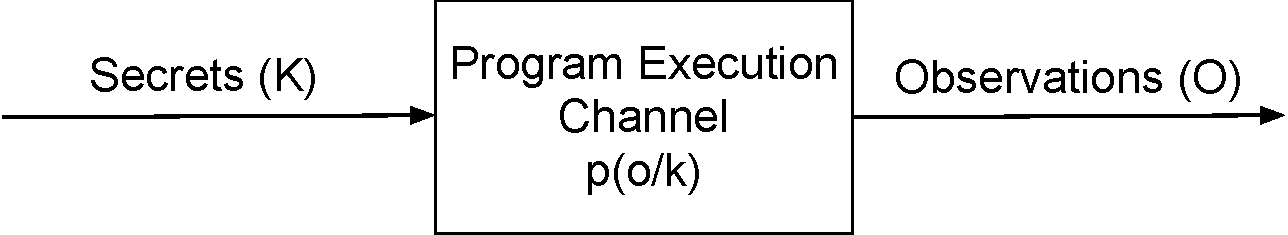
\includegraphics[width=\columnwidth]{./figures/chapter5/channel.pdf}
    \caption{The relationship between the side-channel attack and the channel capacity. For a deterministic program, the side-channel attack can be seen as the communication between the observation ($o \in O$) and the secret ($k \in K$) via a discrete memoryless channel.}
    \label{fig:side_channel}
\end{figure}

With the above definitions, we define the following mapping between $\beta$,
$K$, $M$, and $O$:

\begin{displaymath}
    \beta(K, M) \rightarrow O
\end{displaymath}


Side-channel attacks can be seen as a process that refers the secret ($K$) based on the observations ($O$) shown in the figure~\ref{fig:side_channel}. As an attacker, he can observe the memory address of the victim program. He wants to infer the original secret ($k$) based on the observation. We also assume the attacker knows the known message $m \in M$. In the rest of paper, we use $\beta(K) \rightarrow O$ to denote a victim program with side-channel vulnerabilities.

\section{Method}
In this section, we first provide two examples shows how we rank the side-channel vulnerability. After that, we prove that our method is the conservative estimate of the amount of the each leakage.

\subsection{An Example}
Figure~\ref{fig:example1} show a function that is vulnerable to side-channel attacks. The function take a input secret from the caller. Depending on the value of the secret, it may access different values at line 7. Suppose an attacker can observe which item in the table \textsf{T} is accessed, he can infer the secret based on the observation.
\begin{figure}[h]
\begin{minipage}{0.6\linewidth}
\begin{lstlisting}
void bar(uint8_t secret)
{
  uint8_t T[128];
  uint8_t index = 0, t;
  int i;
  index = (index+secret)%128;
  t = T[index];
  ...
}
\end{lstlisting}
\end{minipage}
\hspace{-4pt}
\hfill
\hspace{-4pt}
\begin{minipage}{0.45\linewidth}
\resizebox{\textwidth}{!}{%

\begin{tabular}{cccccccccc}
\toprule
\diagbox{S}{T} & 0 & 1 & 2 & 3 & 4 & 5& 6& 7 &  ...\\ 
\midrule
0 & A &  &  &  &  &  \\
1 &  & A &  &  &  &  \\
2 &  &  & A &  &  &  \\
3 &  &  &  & A &  &  \\
4 &  &  &  &  & A &  \\
5 &  &  &  &  &  & A & \\
6 &  &  &  &  &  & &A \\
7 &  &  &  &  &  &  && A\\ 
\bottomrule
\end{tabular}%
}
\end{minipage}
\caption{A Serious Leakage}\label{fig:example1}
\end{figure}

To assess the sensitive level of the vulnerability, we use the sampling method to estimate the leakage. Suppose we give the function input from $0, 1, \dots, 7$ and observe the array $T$, we can find each different input have one unique observation. Therefore, the secret can be uniquely determined.

\begin{figure}[h]
\begin{minipage}{0.60\linewidth}
\begin{lstlisting}
void bar(uint8_t secret)
{
  uint8_t T[128];
  uint8_t index = 0, t;
  int i;
  index = (index+secret)%128;
  t = T[index % 4];
  ...
}
\end{lstlisting}
\end{minipage}
\hspace{-4pt}
\hfill
\hspace{-4pt}
\begin{minipage}{0.45\linewidth}
\resizebox{\textwidth}{!}{%

\begin{tabular}{cccccccccc}
\toprule
\diagbox{S}{T} & 0 & 1 & 2 & 3 & 4 & 5& 6& 7 &  ...\\ 
\midrule
0 & A &  &  &  &  &  \\
1 &  & A &  &  &  &  \\
2 &  &  & A &  &  &  \\
3 & &  &  & A &  &  \\
4 & A &  &  &  &  &  \\
5 &  &  A& &  &  & & \\
6 &  &  & A &  &  & & \\
7 &  & &  &  A&  &  && \\ 
\bottomrule
\end{tabular}%
}
\end{minipage}
\caption{A Minor Leakage. }\label{fig:example2}
\end{figure}
On the other hand, the second example also have a side-channel leakages at line 7. However, the leakage is slightly different. Still, we test the program with input from $0, 1, \dots, 7$. However, we find the attacker can not uniquely determine the secret based on the observation of table $T$. For example. both $0$ and $4$ read the first the item of the table. Therefore, we think the vulnerability is slightly minor than the previous one. Here comes with the definition of the amount of leaked information of the vulnerability.

\begin{mydef}
    \label{def}
    Suppose we have a program $\beta$ with the input set $K$. We randomly select $k_1, k_2, \dots, k_n \in K' \subseteq K$ as the input. We denote it as
    $$\beta(K') \rightarrow	O'$$

    Here $O$ is a set that consists of various observations $o_1, o_2, \dots, o_m$. The amount of leaked information $L_{\beta(K')\rightarrow O'}$ based on the observation ($o$) is
    $$L_{\beta(K')\rightarrow O'} = H(O') $$
\end{mydef}


With Definition~\ref{def}, we can calculate the information leakage in Figure~\ref{fig:example1} and Figure~\ref{fig:example2} respectively. In Figure~\ref{fig:example1}, we have $8$ kinds of observations and each observation is uniformly distributed. Therefore, the information leakage is $log_2{8} = 3$ bits. In Figure~\ref{fig:example2}, we have $4$ kinds of observations and each observation is also uniformly distributed. Therefore, the information leakage is $log_2{4} = 2$ bits. We test the program with $8$ inputs. Therefore, the Shannon entropy of the original K $H(K)$ is also $3\,\mathrm{bits}$, according to Equation~\ref{eq1}. Therefore, the leakage in Figure~\ref{fig:example1} show the leakage is leaked totally.

\subsection{A Conservative Estimation}
In this section, we prove Definition~\ref{def} is the conservative estimation of the amount of leaked information based on the channel capacity. 

\begin{theorem}\label{the1}
If an attacker launches a side-channel attack on  deterministic programs, then the channel between the secret and the observation is a noiseless loss channel.
\end{theorem}

\begin{myprof}
According to information theory,
\begin{align*}
     I(K;O) & = H(O) - H(O|K) \\
            & = H(O) - \sum_{k {\in} K }{p(o|k)\log_2p(o|k)}
\end{align*}
For a deterministic program, $p(o|k)=1$. As a result, $H(O|K) = 0$.
\begin{align*}
     C(K;O) = \max_{p(k)} I(K;O) = \max_{p(k)} H |O| 
\end{align*}
\end{myprof}

With THEOREM~\ref{the1}, we can have
\begin{align*}
     \max_{p(k)} H |O| >= \max_{p(k')} H |O'| >= H |O'|
\end{align*}

Accordingly, if Definition~\ref{def} says the vulnerability leakage has $m$ bits of leakages, then the vulnerability can have at least $m$ bits of leakages. We can use the definition to detect those severe leakages. In the examples of Figure~\ref{fig:example1} and Figure~\ref{fig:example2}, because the input secret range from $0$ to $255$, we can calculate the precise value of the amount of information leakage by iterating each input keys. In Figure~\ref{fig:example1}, each item in the array could be read. Therefore, the channel capacity in Figure~\ref{fig:example1} is $\log_2{128} = \,7\, \mathrm{bits}$. In Figure~\ref{fig:example2}, there could be $4$ kinds of information, so the information leakages defined by channel capacity is $\log_2{4} = \,2\, \mathrm{bits}$. Compared with the result from Definition~\ref{def}, we can see that the amount of leakages by Definition is a conservative estimation.

\section{Align Non-deterministic Address Access Across Multiple Executions}
We compare address accesses of different executions generated by different inputs to quantify the amount of leakage information. A meaningful comparison requires we align executions across multiple runs before we quantify the leakage. In this work, we combine the information from both the source code and the binary executable to align the memory access during the execution.


\begin{figure}[h]
\begin{minipage}{0.45\linewidth}
\begin{lstlisting}[numbers=none]
uint8_t *T = malloc(4);
if (T==NULL) exit(1);
...
t = T[i];    
\end{lstlisting}
\end{minipage}
\hfill
\begin{minipage}{0.6\linewidth}
\resizebox{\textwidth}{!}{

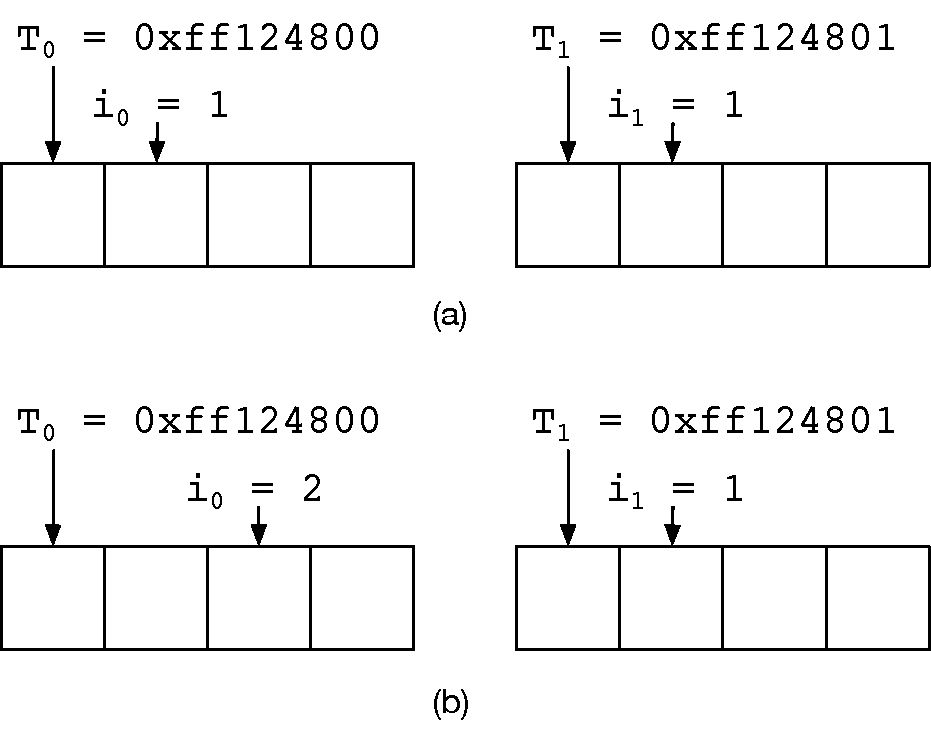
\includegraphics[width=\columnwidth]{./figures/chapter5/align.pdf}

}
\end{minipage}
\caption{Without proper address alignment, there could be many false positives and false negatives.}\label{fig:align}
\end{figure}

Considering the example in figure~\ref{fig:align}, it read the data from the array \textsf{T} based on the index (i). If the index (i) is associated with a key, it could be a side-channel vulnerability. Unlike the example in the previous section, the array \textsf{T} is on the heap. Data on the heap are allocated in different addresses each time. Suppose during the first run, \textsf{T} is allocated at the address \textsf{0xff124800} and \textsf{T} is allocated at the address \textsf{0xff124801} at the second run. For the example in Figure~\ref{fig:align}(a), the index that used to access the array is always $1$, so it should not be a side-channel vulnerability here. However, because the based address is different. So we get two different memory accesses. Under the circumstance, it is a false positive. Besides, it can cause false negatives as the example shown in Figure~\ref{fig:align}(b). In the example, different keys lead to different index. However, as $T_0 + i_0$ equals to $T_1 + i_0$, \tool{} can not observe the difference here, which can cause a false positive.

\textbf{Our Strategy: } We assign a value for each memory location~\cite{sumner2010memory}. The value should satisfy the following characteristics. 
\begin{itemize}
\item \textbf{Uniqueness.} At any point during the execution, different memory cells must have a different value.
\item \textbf{Alignment.} The same memory cell across multiple executions should share the same value.
\end{itemize}

There are some possible solutions that can assign the value.
\textbf{Run-time Information.} One example here is the concrete memory address during the runtime. Such a value satisfy the uniqueness characteristic. However, as the example shown in Figure~\ref{fig:align}, it does not have the alignment property.
\textbf{Source Code Information.} Alternatively, we can use the information from the source code. Recent work~\cite{sumner2010memory} proposes using the execution point that allocate the memory cell as the index and tracking the pointer arithmetic to track the pointer that points to the memory. However, such a method may miss the alias symbol that points to the same memory cell.

We propose to combine both the information from the source code and the runtime to align the memory access during the execution. At the point the memory is allocated, we use the tuple $(start\ address, length)$ to represent the buffer. In the following execution, we check if any memory access falls into the range of those tuples. If so, we add the memory access into the tuple. After the execution, the tuple can be mapped into the location of the source code and we only compare the memory access that belongs to the same lines in the source code.

\section{Design}
In this section, we explain the implementation of \tool{}.
we first present the overview of \tool{}. After that, we discuss some design details to implement \tool{}.

\subsection{Overview}
Figure~\ref{fig:workflow} shows an overview of our side-channel leakages quantification tool. Given the source code of the victim program, \tool{} can find the address-based side-channel leakages by fuzzing the victim program. To assist the illustration, we divide the workflow of ~\tool{} into three steps. For the first step, we build the target program from the source code. After that, we give them random inputs to the victim program and run the target program and record each of the address in the binary file is hit or not and store the information in a bitmap. Next, we analyze the side-channel leakage from the address access bitmap. We split the address space into several segments to speed up the comparison according to Meta information. Finally, \tool{} Generate the final leakage report. For each leakage sites, \tool{} gives the conservative estimation of the information leakage. Every leakage site in the report is a true leakage and there is no false positives.

\begin{figure}[ht]
    \centering
    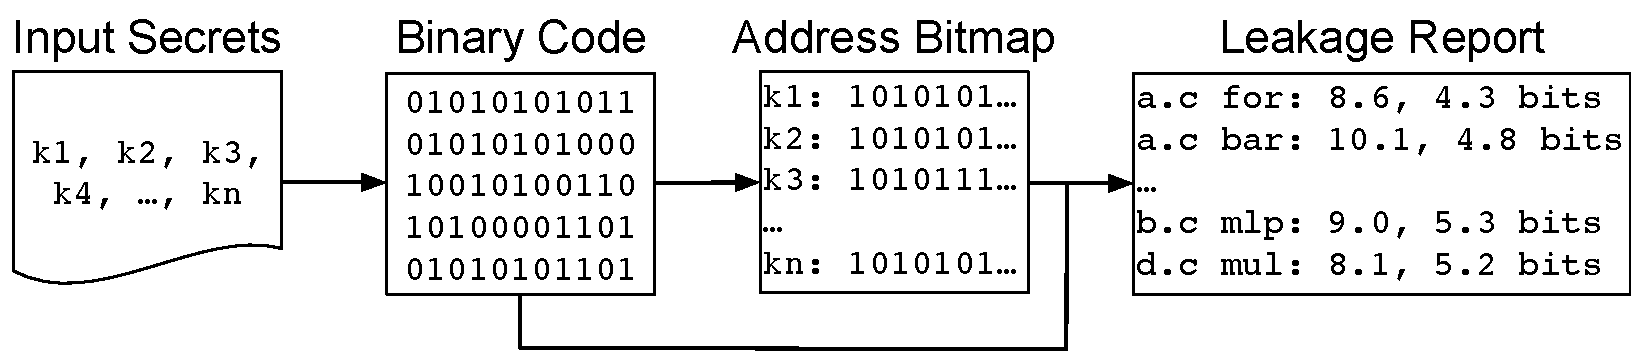
\includegraphics[width=\columnwidth]{./figures/chapter5/workflow.pdf}
    \caption{The workflow of \tool{}. We try to divide the \tool{} into three steps to assist the illustration. }\label{fig:workflow}
\end{figure}

\subsection{Step 1: Fuzzing}
After we build the software into the binary executable, we give the binary code the random inputs. For cryptography libraries, the input is the encryption key. For non-cryptography libraries, the input could be images, text, and information in other format. Encryption algorithms like AES, DES take an array representing the secrets. We generate the random input by flipping the each bit of the keys. Some other programs also takes an buffer as the input. The buffer may contains the redundancy information and follow a specific format. So not any input that satisfies the input length is a valid input. Under the circumstance, we have a dictionary that contains the input. For example, Crypto libraries usually take PKCS \#1 as the input of RSA private key. We use some other tools to generate a list of valid keys and use the key to sample the program. Due to the enormous search space, we can not iterate every inputs. However, our method can give the conservative  estimate of each leakage site. 
\subsection{Step 2: Address Record}
Next, we record the memory access information based on the input secret. We use the dynamic binary instrumentation (DBI) tool to record the whether a particular memory access information is accessed or not. Inspired by the AFL and valgrind, we use the bitmap to represent whether a particular memory is accessed or not. For example, the bitmap ${0101}$ of address $address_1, address_2, address_3, address_4$ means that $address_2, address_4$ are hit during the execution. During the execution, the direct information we get is the virtual memory address (VMA). However, we transfer the address into the offset (Load Memory Address (LMA)) in the original binary file. It has two benefits. First, modern computer systems employ the the Address Space Layout Randomization (ASLR). With ASLR, the operating system randomly put the enclave code and data at various memory offset. As a result, even for the same input, the code will get different execution traces because the enclave image is loaded at a different address each time Second, it helps us find the leakage site in the source code.

We rely on the program header and symbol information to recover the offset in the binary. During the loading process, the operating system maps each segment into a continuous memory region. So the offset of the virtual memory address between the code within the same segment is the same as the offset within the binary file. We choose the start address of some common functions (e.g, $main$) ($b$) as the navigation function. We get the virtual memory address of the start of the function ($\mathit{VMA_b}$) from the DBI tool and the load memory address of the function ($\mathit{LMA_b}$) from the symbol information. For any virtual address, we use Equation~\ref{equ:eq6} to calculate the offset in the original address.
\begin{equation}\label{equ:eq6}
    \mathit{LMA_a} = \mathit{LMA_b} - VMA_b - VMA_a
\end{equation}

There are two kinds of memory access: the access to the code and the access to the data. 
\begin{itemize}
\item Code Access. The memory address of the code is the value of $rip$ register. However, the length of x86 instructions can be from 1 byte to 15 bytes. For instructions whose length is longer than one byte, we also update the address  after the value $rip$ until the address reach the boundary of the instruction.
\item Data Access. For instructions with memory access, we identify all the operands of each instruction and. Same as the code address, the instruction can read or write multiple bytes one time.  Instructions like \textsf{push} and \textsf{pop} have implicit memory access. We all update the bitmap of the address correspondingly.
\end{itemize}

\subsection{Step 3: Leakages Detection and Quantification}
In this step, we detect and quantify the side-channel leakage. For each $k \in K$, we have a boolean number ($0$ or $1$) to describe whether the address $addr$ is accessed or not during the execution when the input is $k$. For the brevity of description, For the brevity of description, we use $B^{addr}_{k_i}$ to denote the boolean number. 



\subsubsection{Various Granularities Side-channel Detection}
\tool{} can detect the side-channel vulnerabilities in different granularity. For each granularity, we calculate a new bitmap that represents access information of each unit. We have the bitmap of the memory access at the byte level. An attacker who has the coarse-grained observation at address space may not be able to distinguish the address difference. For example, modern X64 computer system uses 48-bit virtual memory addresses. The top 36 bit of the virtual address is called Virtual Page Number (VPN) and the bottom 12 bits of the virtual address is called offset. The memory management unit (MMU) transfer the virtual address into the physical address by mapping the Virtual Page Number (VPN) into the Physical Page Number (PPN) while keep the offset of the address. So two addresses with the Same VPN but different offset are not distinguishable by an attacker who only has the the page-level observation. 

Suppose a program reads one byte at memory $\mathsf{0x7ffff7ffd001}$ when the secret is $k_1$ and reads a different byte at memory $\mathsf{0x7ffff7ffda01}$ when the secret is $k_2$, an attacker who has the page-level observation can not launch the attack but an attacker who launches the cache attack can know the input is $k_1$ or $k_2$. We update the new bitmap of the large unit by merging the bitmaps of small units that fall into the large unit. That is, $\forall addr_1, addr_2, \dots, addr_n \in addr_N, B^{addr_N}_{k_i} = B^{addr_1}_{k_i} \lor,\dots,\lor B^{addr_N}_{k_n}$.


\subsubsection{Leakage Detection} The access of the address is secret-dependent if $ \exists\, k_{i1}, k_{i2} \in K, \, B^{addr}_{k_i1} \oplus  B^{addr}_{k_i2} =1 $. In the paper, we perform the logical exclusive OR operation on every boolearn value in the same address. If the result is $1$, then the address is vulnerable to the side-channel attacks.

\begin{myexample}
Suppose we sample a program from $k1$ to $k8$ and record the memory access at the granularity of each byte from $\mathsf{7ffff7ffd000}$ to $\mathsf{7ffff7ffd03f}$ (One cache line), we perform the bit-wise or operation of each address with the address range. Because the cache line is always accessed. We think it is not a leak here.
\begin{center}
\begin{tabular}{c}
{
\begin{lstlisting}[frame=none]
              k1  k2  k3  k4  k5  k6  k7  k8   Result  
7ffff7ffd000   1   0   1   0   1   1   0   1 
7ffff7ffd000   0   1   1   0   1   1   1   1 
7ffff7ffd000   1   1   1   1   1   1   0   1 
7ffff7ffd000   1   0   1   0   1   1   1   1 
...
7ffff7ffd03f   1   0   1   0   1   1   1   0  
cache line     1   1   1   1   1   1   1   1    0 (No Leaks)
\end{lstlisting}
}
\end{tabular}
\end{center}
\end{myexample}

\subsubsection{Estimate The Leaked Information}
According to Definition~\ref{def}, we quantify the information leakage based on the distribution of the observation. If we calculate the information leakage from an $4MB$ memory area, then the length of the byte-level bitmap is $4*1024*1024 = 4194304$. While it is possible to compute the distribution of the bitmap theoretically, it is hard to compare the bitmap of such length in practice.

To solve the problem, we use the debug information to split the bitmap into several segments and map the leakage site into the location of the source code. Each segment maps the address access situation of the function in the source code. In our setting, the max length of the bitmap of each segment is $1024$, the length of \textsf{uint1024\_t}. So we can put the bitmap into a variable. The split operation ease the computation. But it also adds the limitation of max address range when we quantify the side-channel leakage shown in Table~\ref{tab:size_limitation}. We think the range of the memory is big enough for us to quantify the most of the cache side-channel attacks. 

\begin{table}[h]
    \centering
\resizebox{0.45\textwidth}{!}{%

\begin{tabular}{llll}  
\toprule
Granularity  & Byte & Cache Line (64 Bytes) & Memory Page (4 KB) \\
\midrule
Range & 1024 Bytes & 64 KB  &  4 KB \\
\bottomrule
\end{tabular}
}
    \caption{The maximum range address range when we quantify the amount of the leakage with different granularity.}
    \label{tab:size_limitation}
\end{table}

After that, we traverse the bitmap for each $k$ and count it to get the distribution of the bitmap. The counting process is like traversing a binary tree. 

\begin{myexample}
Shown in Figure~\ref{fig:design:example2}, we have the following observation from $k_1$ to $k_8$, then we count the distribution of  the observation. The process is like traversing a binary tree and increase the counter of the child node. According to Definition~\ref{def}, the amount of the leakage is 

\begin{displaymath}
  H(O') = - \frac{3}{8}*\log_2{\frac{3}{8}}- \frac{1}{2}*\log_2{\frac{1}{2}}
  - \frac{1}{8}*\log_2{\frac{1}{8}} = 1.4 \,\mathrm{bits}
\end{displaymath}

\begin{figure}[h]
\begin{minipage}{0.4\linewidth}
\resizebox{\linewidth}{!}{
  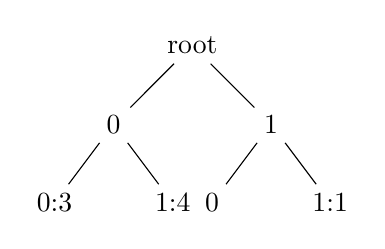
\begin{tikzpicture}
  [level distance=1cm,
  level 1/.style={sibling distance=2cm},
  level 2/.style={sibling distance=1.5cm}]
  \node {root}
    child {node {0}
      child {node {0:3}}
      child {node {1:4}}
    }
    child {node {1}
    child {node {0}}
      child {node {1:1}}
    };
\end{tikzpicture} 
 
}\end{minipage}
\hfill
\begin{minipage}{0.18\linewidth}
{
\begin{lstlisting}[frame=none, numbers=none]
k1  00
k2  01
k3  01
k4  01
k5  00
k6  01
k7  11
k8  00
\end{lstlisting}
}
\end{minipage}
\hfill
\begin{minipage}{0.30\linewidth}
\resizebox{\linewidth}{!}{

\begin{tabular}{ll}  
\toprule
Observation  & P  \\
\midrule
00 & $3/8$   \\
01 & $1/2$   \\
10 & 0 \\
11 & $1/8$\\
\bottomrule
\end{tabular}
}
\end{minipage}
\caption{Example 2}\label{fig:design:example2}
\end{figure}
\end{myexample}


\section{Implementation}
We have implemented a prototype of \tool{}. It takes an input of ELF binary as well as the source code of the corresponding problem. The front-end of \tool{} is implemented in Python. It can generate random inputs and test the program with those inputs many times.  The address record part is implemented as an Intel Pin tool plugin in C++ to record the bitmap for each input. The main component uses libelfin, an open source library to parse ELF binaries and read DWARF debug information. The current implementation can support both 64-bits and 32-bits ELF binary in Linux. \tool{} will be open-sourced.

\section{Discussion}

This paper presents an approach that tries to give the conservative estimate of the amount of leaked information by address-based side-channel attacks. Those attacks exploit the data-flow from secrets to load address and the data-flow from the data-flow from secrets to branch conditions to retrieve secrets based on the observation on the memory accesses. Despite those kinds of side-channel leakages have been discovered for decades, the up-to-date software still has some side channel leakages. For some of those vulnerabilities, developers don't fix them because they think those side-channel vulnerabilities are not important. To show the importance of those side-channel leakages, one way is to demonstrate an end-to-end attack based on the vulnerability. However, demonstrating an end-to-end attack often need a lots of manual efforts and the domain knowledge of the victim program, which is not often the case in practices. It is good to have a tool that can assess the severity level of those side channel leakages automatically. So it would be better to have a proper metric to quantify the side-channel leakage. However, we find previous side-channel quantification tools are developed to  ensure the noninterference of the program. They use over approximation heuristics method to quantify the leakage. For example, CacheAudit estimate that a 128-bit AES encryption can leaks more than 128 bits. As a result, even those tool reports severe leakage, it does not mean the program has a truly severe leakage.

Our tool can give the conservative estimation of the side-channel leakage based on Channel Capacity. The channel capacity measures  the information flow between the source and the destination. One useful characteristic of channel capacity is not affected by the distribution of the input, which is useful because in practice we can not have an assumption on the input secrets of the software. In the paper, we use the sampling result to over approximate the true value of the channel capacity. We prove the sampling method presented in the paper can only give the conservative estimation of the amount of the true leakage.

\subsection{Limitation}
\tool{} is a dynamic approach. So it bears the same limitations of dynamic approaches as well. \tool{} may have the coverage problem and can miss some side-channel vulnerabilities. It is usually not a crucial problem for cryptography libraries as cryptography libraries are designed to have the same control-flow with various inputs. For other libraries like graphic rendering, machine learning, \tool{} is very likely to miss some side-channel vulnerabilities. However, \tool{} is not designed to find side-channel vulnerabilities. The goal of \tool{} is to pick up those really serious side-channel vulnerabilities from the numerous vulnerabilities. So we do not think it is a main limitation of \tool{}. However, users of \tool{} should be aware the code coverage problem. 

Another limitation is that \tool{} can only find the position in the code that leaks the sensitive information, but it is not the root cause of the leaks. Consider the example in Figure~\ref{fig:limitation}, it takes the secret as the input. At line 3, it calculate an index based on the value of the secret. Depending on the value of index, it may or may not run the code at line 6. So line 5 is the reason that causes the vulnerability. But \tool{} can only tell the line 6 can leak the information, despite it is not the root cause of the vulnerability. 

\begin{figure}
\centering
\begin{lstlisting}[xleftmargin=.02\textwidth,xrightmargin=.01\textwidth]
int foo(uint8_t secret){
  uint8_t index = 0, t;
  index = (index+secret)%128; // The index contains secrets
  ...
  if(index == 0){             // Secret-dependent flows
    bar(r, x, n)              // The observation
  }
  ...
}
\end{lstlisting}
    \caption{A code fragment}
    \label{fig:limitation}
\end{figure}
